\documentclass[a4paper]{article}
\usepackage{a4,amsmath,amssymb}
\usepackage[usenames]{color}
\usepackage{graphicx}
\usepackage{verbatim,url}
\usepackage{contour}
%\usepackage{rotating}

\setlength{\textwidth}{\paperwidth}
\setlength{\oddsidemargin}{0cm}
\setlength{\marginparsep}{0cm}
\setlength{\marginparwidth}{0cm}
\setlength{\textheight}{50cm}
\setlength{\headheight}{0cm}
\setlength{\voffset}{-1in}
\setlength{\hoffset}{-1in}
\setlength{\topmargin}{0cm}
\setlength{\headsep}{0cm}
\setlength{\tabcolsep}{0.2em}

\newcommand{\buh}[1]{\contour{white}{\textsf{#1}}\\}
\newcommand{\bah}[1]{\textsf{#1}\\}
%\textcolor{my}{#1}}\\}

%\makeatletter
%\addto@hook\every@verbatim{\textbf}

\begin{document}
\contourlength{1pt}
\contournumber{20}
\definecolor{my}{rgb}{1,1,1}
\definecolor{img}{rgb}{0.6,0.6,0.6}
\color{black}
\begin{center}
\mbox{}\\
\vspace{-1.5cm}
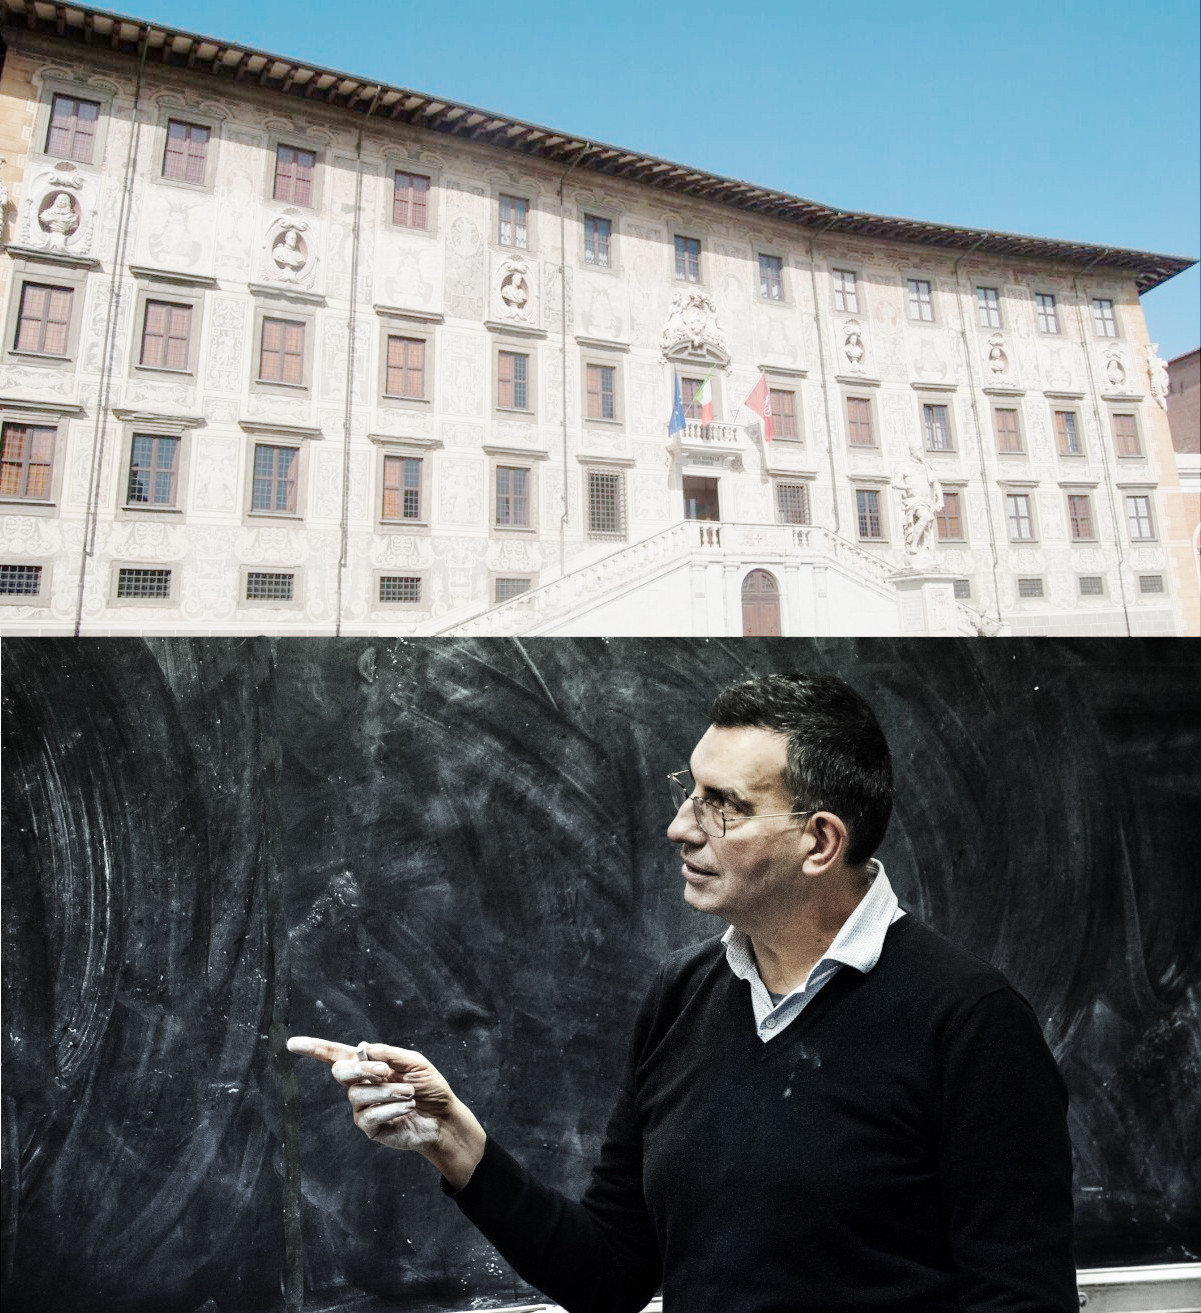
\includegraphics[scale=0.70]{sfondo.jpg}
\\
\vspace{-31cm}
%\mbox{}\raisebox{-11cm}[0pt][0pt]{\mbox{}\hspace{-11cm}\color{img}\input{cv}}
%\mbox{}\raisebox{-10cm}[0pt][0pt]{\mbox{}\hspace{10cm}\color{img}\input{pde}} 
\bigskip
\Huge
\buh{}
\large
\buh{}
\bigskip
\bf

\Huge
\buh{CALCULUS of VARIATIONS}
\buh{\&}
\buh{GEOMETRIC MEASURE THEORY}
\vspace{2cm}
\Large
\buh{Aula Magna --- Polo Fibonacci}
\vspace{2cm}
\huge
\buh{Pisa, June 12--16, 2023}
\Large
\bigskip
\buh{The meeting will be the opportunity to celebrate the 60th birthday of Luigi Ambrosio}
\end{center}
\color{my}
\vspace{3cm}
\mbox{}\hspace{1cm}
\begin{minipage}{0.45\textwidth}
\Large
\bah{Invited Speakers:}
\\
\normalsize
\textsf{
Giovanni Alberti (Università di Pisa)\\
Andrea Braides (SISSA Trieste)\\
Yann Brenier (École normale supérieure Paris)\\
Giuseppe Buttazzo (Università di Pisa)\\
Xavier Cabré (ICREA and \mbox{Universitat~Politècnica~de~Catalunya)\hspace{-3cm}\mbox{}}\\
Piermarco Cannarsa (Università di Roma Tor Vergata)\\
Maria Colombo (EPFL Lausanne)\\
Gianni Dal Maso (SISSA Trieste)\\
Guido De Philippis (New York University)\\
Alessio Figalli (ETH Zürich)\\
Irene Fonseca (Carnegie Mellon University)\\
Nicola Fusco (Università di Napoli Federico II)\\
Adriana Garroni (Università La Sapienza Roma)\\
Nicola Gigli (SISSA Trieste)\\
Shouhei Honda (Tohoku University)\\
Carlo Mantegazza (Università di Napoli Federico II)\\
Simon Masnou (UCBL Lyon)\\
Andrea Mondino (University of Oxford)\\
Diego Pallara (Università del Salento)\\
Giuseppe Savaré (Università Bocconi, Milano)\\
Francesco Serra Cassano (Università di Trento)\\
Dario Trevisan (Università di Pisa)\\
}
\end{minipage}
\vspace{1.4cm}
\hspace{4cm}
\begin{minipage}{0.45\textwidth}
    \vspace{7cm}
    \Large
    \bah{Organizers:}
    \\
    \normalsize
    \textsf{
        Matteo Focardi\\
        Valentino Magnani\\
        Matteo Novaga\\
        Emanuele Paolini\\
        Aldo Pratelli
    }\\
    \end{minipage}
\\
    \mbox{}\hspace{1cm}
    \begin{minipage}{2cm}
    {\mbox{\hspace{-0.2cm}}\tiny\texttt{la2023.cs.dm.unipi.it}}\\
    \includegraphics*[height=1.5cm]{qr-bw.png}\mbox{}
    \vspace{1.2cm}\mbox{}
    \end{minipage}
    \noindent
    \hspace{0.5cm}
    \includegraphics*[height=1.3cm]{matematica_dx_bianco.pdf}
    \hspace{0.1cm}
    \includegraphics*[height=1.5cm]{marchio_unipi_orizz_white.png}
    \mbox{}\hspace{0.5cm}
    \includegraphics*[height=1.5cm]{Sns-Scuola-Normale-Superiore-Pisa.png}
    \hspace{0.5cm}
    \includegraphics*[height=1.6cm]{logo_DIMAI_positivo-1-300x150.png}
    \mbox{}
\end{document}